\input{preamble}

\begin{document}

\header{3}{3D Ray Tracing}

Our previous homework renders images using the ``rasterization'' algorithm. In this homework we will explore an alternative called ``ray tracing''. Ray tracing, while having the reputation of being more advanced, is actually mostly simpler than rasterization. The catch is performance. Despite significant improvement of ray tracing performance in the past decade, for objects directly visible from the camera, rasterization is still faster due to better cache locality. On the other hand, ray tracing enables more general effects and complex geometry in much simpler ways. For example, in this homework we will implement spherical geometry, hard shadow and mirror reflection. We will explain the nuance in the lectures.

Our homeworks are inspired by the book \href{https://raytracing.github.io/}{Ray Tracing in One Weekend (RTOW)} (click the link for free access of the e-book). Feel free to read the book and even reuse their code. A verbatim copy probably will not work anyway. 

\paragraph{Antialiasing.} In this homework we still don't do antialiasing. Test the pixel center.

\section{Rendering multiple spheres (15 points)}
We will start with rendering of spheres. You will notice that we advance slightly faster than before because supposedly you have been trained well by the previous homework. 

\begin{figure}[h]
    \centering
    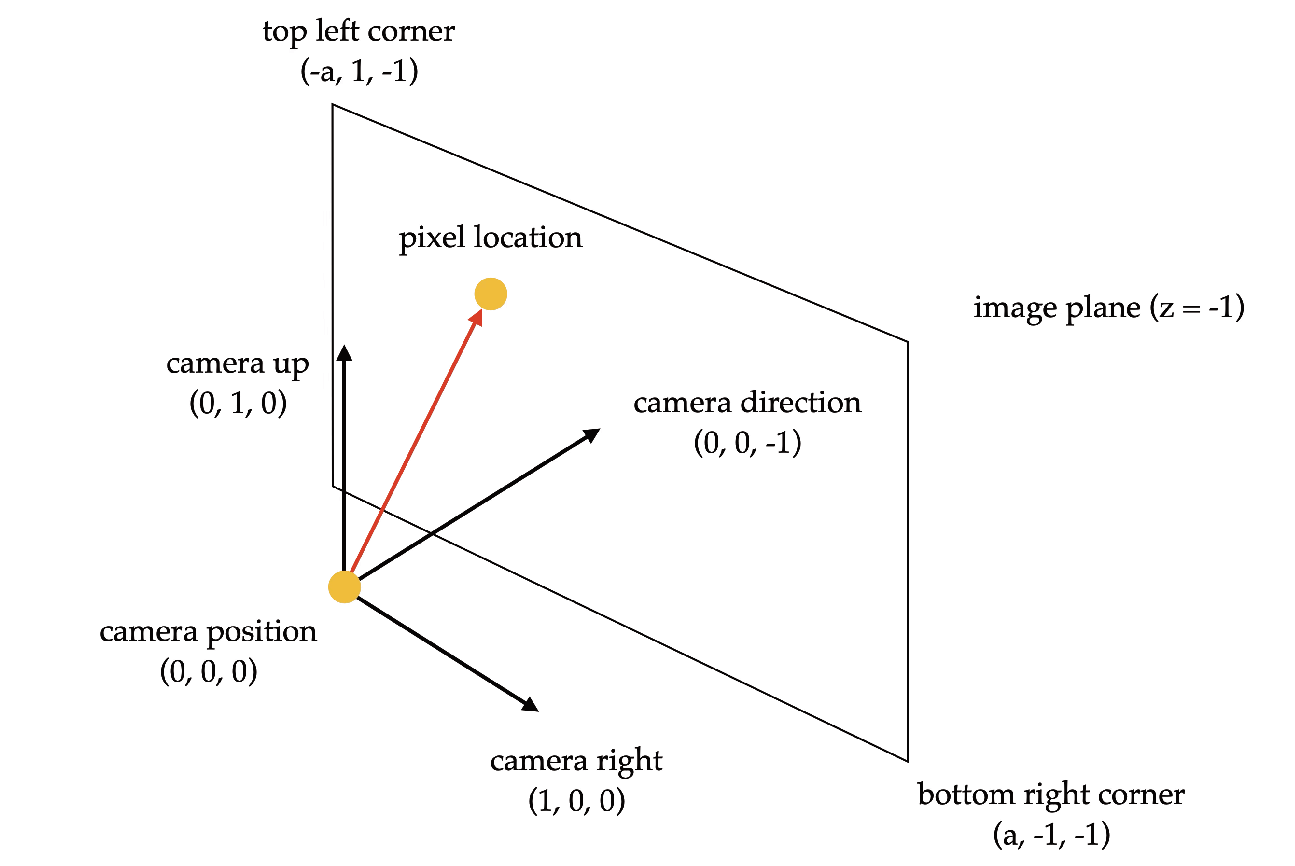
\includegraphics[width=0.5\linewidth]{imgs/ray_casting.pdf}
    \caption{The camera space coordinates of the image plane for Homework 3.1. $a$ is the aspect ratio (width / height). We shoot a ray from the origin $(0, 0, 0)$ with direction towards a pixel location on the image plane, with the plane located at $z=-1$ (this means that the ``focal length'' is $1$). We assume the field of view is 90 degree in this part. In this case, the top left of the image plane is $(-a, 1, -1)$ and the bottom right is $(a, -1, -1)$. We can use this geometry to figure out the exact location of the pixel center.}
    \label{fig:raycast}
\end{figure}

The idea of ray tracing is to shoot rays from the camera origin, towards pixel on the image plane. \cref{fig:raycast} illustrates the idea. In HW 3.1-3.3 we are going to assume a fixed camera coordinate system with $x$ points towards right, $y$ points towards up, and $-z$ points into the screen. In HW 3.4 we are going to implement transformation and animation as usual.

After we send out a ray using \cref{fig:raycast}'s geometry, we need to intersect with the scene geometry. For 3.1-3.4 we will assume the scene is solely consisted of spheres. To intersect a ray ($\mathbf{o} + t \mathbf{d}$) and a sphere (center $\mathbf{x}_c$ and radius $r$), we solve the following quadratic equation:
\begin{equation}
	\|\mathbf{o} + t \mathbf{d} - \mathbf{x}_c\|^2 = r^2,
\end{equation}
with $t$ being the only unknown. We have provided a quadratic equation solver \lstinline{solve_quadratic} in \lstinline{hw3_common.slang} that you can use.
Note that a ray can hit the sphere zero, one, or two times. In the case it hits two times, we need to choose the intersection that is closer, while ensuring $t > 0$.

The spheres we will render will be specified in a JSON file. We will share the JSON file with some later parts of the homework, so ignore the information that is irrelevant here like \lstinline{Kd}, \lstinline{Kr}, and \lstinline{lights}:
\begin{lstlisting}[language=json]
{
    "background": [0.5, 0.5, 0.5],
    "objects": [
        {"type": "sphere",
         "center": [0.0, 0.0, -3.0],
         "radius": 1.0,
         "Kd": [0.9, 0.2, 0.2],
         "Kr": [0.0, 0.0, 0.0]}
    ],
    "lights": [
        {"position": [-3.0, 4.0, 1.0], "intensity": [120.0, 120.0, 120.0]}
    ]
}
\end{lstlisting}

Our parser will convert the spheres into a Slang buffer. You can inspect the format in \lstinline{hw3_1.slang} and \lstinline{hw3_common.slang}.

Once we found the closest hit among many spheres, visualize the color using the sphere's normal. But a normal can have negative values, so we need to transform it. Let the normal be $n$, we will visualize $\frac{n+1}{2}$. The background is specified in the scene file.

Your task is to go to \lstinline{hw3_1.slang} and implement the ray tracing process. Test your rendering using the command:
\begin{lstlisting}[language=bash]
	uv run python main.py 3_1 scenes/hw3/single_sphere.json 
\end{lstlisting}

I have put my rendering in \cref{fig:hw3_1}.
\begin{figure}[h]
    \centering
    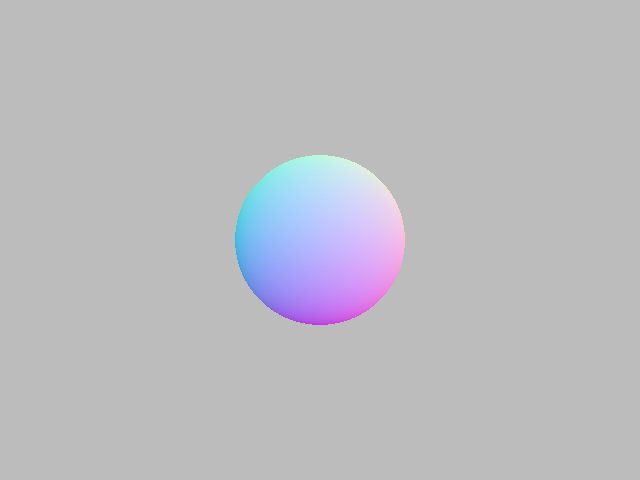
\includegraphics[width=0.5\linewidth]{imgs/hw_3_1.png}
    \caption{Reference rendering for homework 3.1.}
    \label{fig:hw3_1}
\end{figure}

To test your code, we will use these commands:
\begin{lstlisting}[language=bash]
	uv run python main.py -output outputs/hw_3_1_1.png 3_1 scenes/hw3/multiple_spheres.json
	uv run python main.py -output outputs/hw_3_1_2.png 3_1 scenes/hw3/sphere_occlusion.json
	uv run python main.py -output outputs/hw_3_1_3.png 3_1 scenes/hw3/big_sphere.json 
	uv run python main.py -output outputs/hw_3_1_4.png 3_1 scenes/hw3/tangent_spheres.json 
\end{lstlisting}

As usual, send us the images you rendered.

\section{Diffuse lighting and hard shadows (16 points)}
Next we will get rid of the normal visualization and add lighting. We have done lighting in Homework 2, so let us add one more feature: shadows! 

We will use a simple Lambertian shading model for this part. Each sphere will be associated with a \lstinline{Kd} parameter and we light it using multiple point lights in the scene. (Note that we used directional lights in Homework 2. Point lights decay with squared distance.) 

Adding shadow to a ray tracer is super simple: given a point we want to shade and a point light, we simply do an intersection test to find out if there is anything between them! We typically need to set an upper bound $t_{\text{max}}$ for how far a ray can travel. The ray for this intersection test is often called the \emph{shadow ray}. An important detail to handle is self intersection: our shadow ray can intersect with the sphere it starts from due to imperfect floating point math. We avoid self intersection by having a requirement on the minimal $t$ in our intersection routine. Instead of skipping intersections with $t < 0$, we skip over intersection with $t < t_{\text{min}}$. In my implementation, I set $t_{\text{min}} = 10^{-3}$ for all cases. I defined a constant \lstinline{EPSILON} in \lstinline{hw3_common.slang} for you to use. (Note that in Slang, you have to use \lstinline{static const} when defining a global compile-time constant. Otherwise it will be treated as a shader parameter that you need to pass from host code, and will not be initialized.)

To make things more compatible with the later parts of the homework, we use a \lstinline{Shape} structure to store the \lstinline{Kd} parameter and an \lstinline{index} for indexing the spheres array:
\begin{lstlisting}
StructuredBuffer<Shape> shapes
uniform int num_shapes
StructuredBuffer<Sphere> spheres

// accessing the corresponding sphere of the shape
spheres[shapes[i].index]
\end{lstlisting}

That's it! You should be able to get cool images at this point. Go to \lstinline{hw3_2.slang} to implement your ray tracer. Test it using
\begin{lstlisting}[language=bash]
	uv run python main.py 3_2 scenes/hw3/sphere_with_plane.json 
\end{lstlisting}

I have put my rendering in \cref{fig:hw3_2}.
\begin{figure}[h]
    \centering
    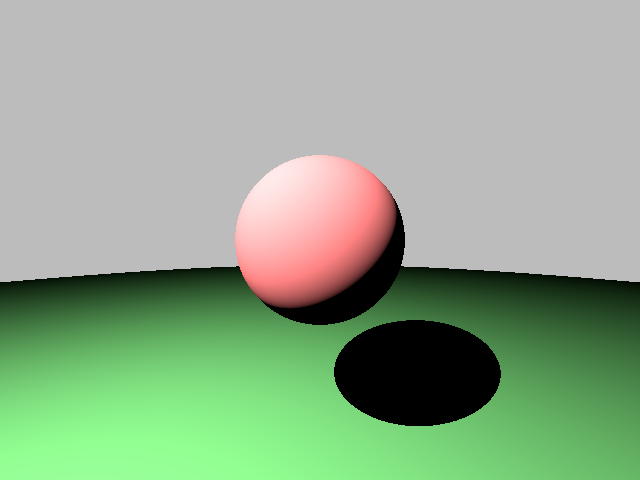
\includegraphics[width=0.5\linewidth]{imgs/hw_3_2.png}
    \caption{Reference rendering for homework 3.2.}
    \label{fig:hw3_2}
\end{figure}

We will grade your renderer using the following commands.
\begin{lstlisting}[language=bash]
	uv run python main.py -output outputs/hw_3_2_1.png 3_2 scenes/hw3/sphere_with_plane_2.json
	uv run python main.py -output outputs/hw_3_2_2.png 3_2 scenes/hw3/two_lights.json
	uv run python main.py -output outputs/hw_3_2_3.png 3_2 scenes/hw3/extra_occluder.json
	uv run python main.py -output outputs/hw_3_2_4.png 3_2 scenes/hw3/rainbow_double_helix.json
\end{lstlisting}

\section{Multiple bounces mirror (16 points)}

Next we will add a mirror reflection effect. For each material, in addition to \lstinline{Kd}, we also have \lstinline{Kr} which is its ``mirror reflection color''. If \lstinline{Kr > 0} for any of the component, then we will need to trace a ray in the mirror reflection direction (using the \lstinline{reflect} function in Slang) to find the reflected color. If a mirror reflection ray doesn't hit any sphere, use the background color.

One unfortunate detail we need to handle: Slang's compute shaders do not universally support recursion, due to hardware constraints. Fortunately it is quite easy to rewrite the mirror reflection recursion into a serial loop. The loop structure looks like this:
\begin{lstlisting}
float3 color = 0.0;
float3 throughput = 1.0;
for (int b = 0; b < max_depth; b++) {
    // compute contribution from point lights
    color += throughput * contribution;
    throughput *= Kr;
    ray = reflect(ray);
}
\end{lstlisting} 
The \lstinline{max_depth} parameter is from our scene to avoid infinite loops.

We also need to be again careful about self intersection. I use the same $t_{\text{min}}$ I used for the shadow ray for the mirror reflection direction intersections.

Go to \lstinline{hw3_3.slang} to implement your ray tracer. Test it using
\begin{lstlisting}[language=bash]
    uv run python main.py 3_3 scenes/hw3/multiple_spheres.json
\end{lstlisting}

I have put my rendering in \cref{fig:hw3_3}.
\begin{figure}[h]
    \centering
    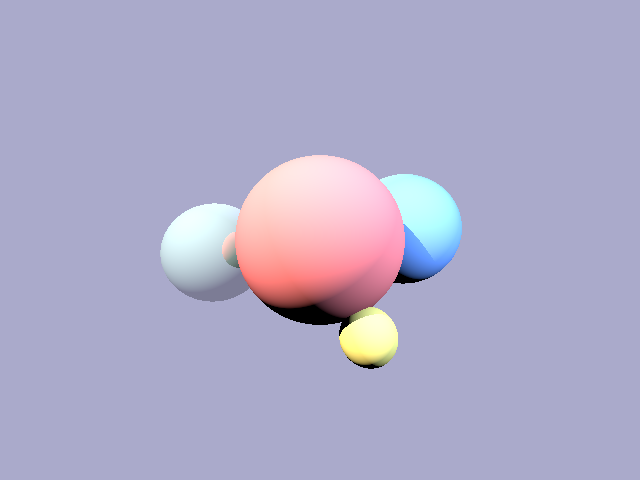
\includegraphics[width=0.5\linewidth]{imgs/hw_3_3.png}
    \caption{Reference rendering for homework 3.3.}
    \label{fig:hw3_3}
\end{figure}

We will grade your renderer using the following commands.
\begin{lstlisting}[language=bash]
    uv run python main.py -output outputs/hw_3_3_1.png 3_3 scenes/hw3/single_mirror.json
    uv run python main.py -output outputs/hw_3_3_2.png 3_3 scenes/hw3/two_mirrors.json
    uv run python main.py -output outputs/hw_3_3_3.png 3_3 scenes/hw3/two_mirrors_2.json
    uv run python main.py -output outputs/hw_3_3_4.png 3_3 scenes/hw3/mirror_ring.json
\end{lstlisting}

\section{Transformation and animation (16 points)}

Next, we will add transformations and animation just like the previous homeworks. Feel free to copy paste the \lstinline{compose_transformations} and \lstinline{interpolate_transformation} from your previous homework into \lstinline{hw3_scene.py}. 

On the Slang side, we need to handle both the camera transformation using \lstinline{Camera::cam_to_world} and \lstinline{Camera::fov_x}, and the object transformation using \lstinline{Shape::world_to_obj} and \lstinline{Shape::obj_to_world}. All the transformations are guaranteed to be affine. The way I do it is: first transform the camera rays to world space using \lstinline{cam_to_world}. Next transform the rays to the object space using \lstinline{world_to_obj}. Next transform the object space intersection points using \lstinline{obj_to_world} and normals using the inverse transpose.

You may find the \lstinline{xform_pt} and \lstinline{xform_vec} functions in \lstinline{hw3_common.slang} useful, though you are not forced to use them. In particular, you need to use \lstinline{mul(M, v)} to do matrix-vector multiplication between matrix \lstinline{M} and vector \lstinline{v}.

For \lstinline{fov_x}, we fix the focal length to be $1$, and \lstinline{fov_x} specifies the horizontal field of view angle in degrees (you can use the \lstinline{radians()} function in Slang to convert it into radians). This means that the width of the image plane is fixed to $2 \cdot \tan(\frac{F}{2.0})$ where $F$ is the FOV in radians, and the height is width divided by the aspect ratio.

One trick that can be very useful is to notice that the intersection $t$ is preserved under affine transformation of the rays, \textbf{provided that we don't normalize the ray direction}. We can show this by applying an affine transformation to $\mathbf{o} + t \mathbf{d}$ and show that the ray remains to be some $\mathbf{o}' + t \mathbf{d}'$ where $\mathbf{o}'$ and $\mathbf{d}'$ are the affine transformation of the origin and the direction respectively. This allows us to reuse the $t$ we compute in the object space across different objects. Again, this only works if we don't normalize the ray direction, and that our ray-sphere intersection code properly handles unnormalized rays.

Go to \lstinline{hw3_4.slang} to implement your ray tracer (remember to copy paste the transformation code on the Python side). Test it using
\begin{lstlisting}[language=bash]
    uv run python main.py 3_4 scenes/hw3/single_sphere_transform.json
    uv run python main.py 3_4 scenes/hw3/single_sphere_animation.json
\end{lstlisting}

I have put my rendering in \cref{fig:hw3_4}.
\begin{figure}[h]
    \centering
    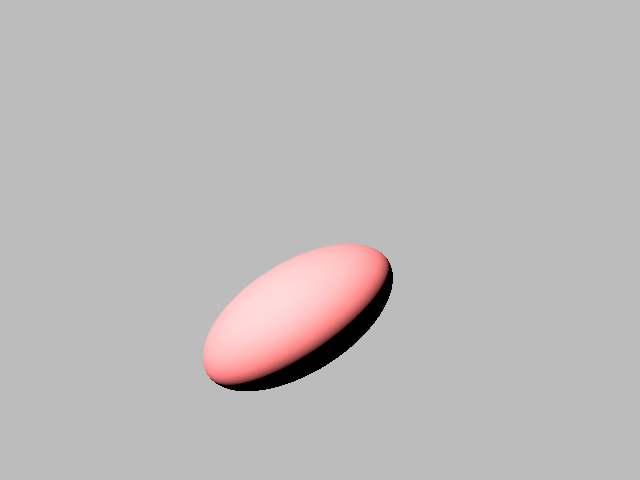
\includegraphics[width=0.5\linewidth]{imgs/hw_3_4.png}
    \caption{Reference rendering for homework 3.4.}
    \label{fig:hw3_4}
\end{figure}

We will grade your renderer using the following commands.
\begin{lstlisting}[language=bash]
    uv run python main.py -output outputs/hw_3_4_1.png 3_4 scenes/hw3/static_transforms.json
    uv run python main.py -output outputs/hw_3_4_2.png 3_4 scenes/hw3/lookat.json
    uv run python main.py -output outputs/hw_3_4_3.png 3_4 -time 4.2 scenes/hw3/bouncing_spheres.json
    uv run python main.py -output outputs/hw_3_4_4.png 3_4 -time 9.3 scenes/hw3/camera_animation.json
    uv run python main.py -output outputs/hw_3_4_5.png 3_4 -time 2.7 scenes/hw3/rainbow_animation.json
\end{lstlisting}

\section{Triangle meshes (16 points)}

Next we will add some triangle meshes! The only difference to the sphere scenes is that now we perform ray triangle intersection, instead of ray sphere intersection! Ray triangle intersection is so well established and so optimized that even experts will just copy paste other experts' code. We already provide the intersection routine invented by Thomas Möller and Ben Trumbore (the famous ``Möller–Trumbore intersection algorithm'') in \lstinline{intersect_tri} in \lstinline{hw3_common.slang} that you can use directly.

The triangle mesh is organized in the following data structure:
\begin{lstlisting}
struct TriangleMesh {
    uint vertex_offset;
    uint triangle_begin;
    uint triangle_end;
    uint bvh_root_index; // Used in 3.6
};

StructuredBuffer<TriangleMesh> meshes
StructuredBuffer<float3> vertices
StructuredBuffer<float3> vertex_normals
StructuredBuffer<uint3> triangles
\end{lstlisting}
We flatten all the triangle meshes' vertices, vertex normals, and face indices into separate contiguous arrays. Given a mesh, we then use \lstinline{triangle_begin} and \lstinline{triangle_end} to loop over all triangles, and use \lstinline{vertex_offset} to look up the corresponding vertex/vertex normal pools. I used something like \lstinline{uint3 tri = triangles[j] + mesh.vertex_offset;} to offset the face indices. Remember to handle transformation and interpolate the vertex normals for both the mirror reflection and the lighting.

Implement your code in \lstinline{hw3_5.slang}. Test it using
\begin{lstlisting}[language=bash]
    uv run python main.py 3_5 scenes/hw3/two_quads.json
\end{lstlisting}

I have put my rendering in \cref{fig:hw3_5}.
\begin{figure}[h]
    \centering
    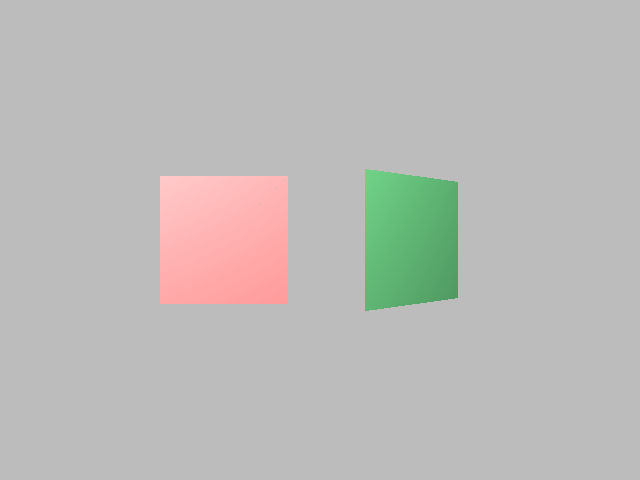
\includegraphics[width=0.5\linewidth]{imgs/hw_3_5.png}
    \caption{Reference rendering for homework 3.5.}
    \label{fig:hw3_5}
\end{figure}

We will grade your renderer using the following commands.
\begin{lstlisting}[language=bash]
    uv run python main.py -output outputs/hw_3_5_1.png 3_5 scenes/hw3/two_quads_2.json
    uv run python main.py -output outputs/hw_3_5_2.png 3_5 scenes/hw3/cube_sphere_sphere.json
    uv run python main.py -output outputs/hw_3_5_3.png 3_5 scenes/hw3/meshes.json
    uv run python main.py -output outputs/hw_3_5_4.png 3_5 scenes/hw3/crystals.json
    uv run python main.py -output outputs/hw_3_5_5.png 3_5 -time 4.5 scenes/hw3/crystals_animation.json
\end{lstlisting}
(For the \lstinline{cube_sphere_sphere} scene: think about why the two spheres look different.)

\section{Bounding Volume Hierarchies (16 points)}
For the last part we will implement an important acceleration using bounding volume hierarchies (BVHs). We will only apply the acceleration to triangle meshes. For each triangle mesh we will build one bounding volume hierarchy, and we will still have a loop to test over all spheres and meshes. 

\begin{figure}[h]
    \centering
    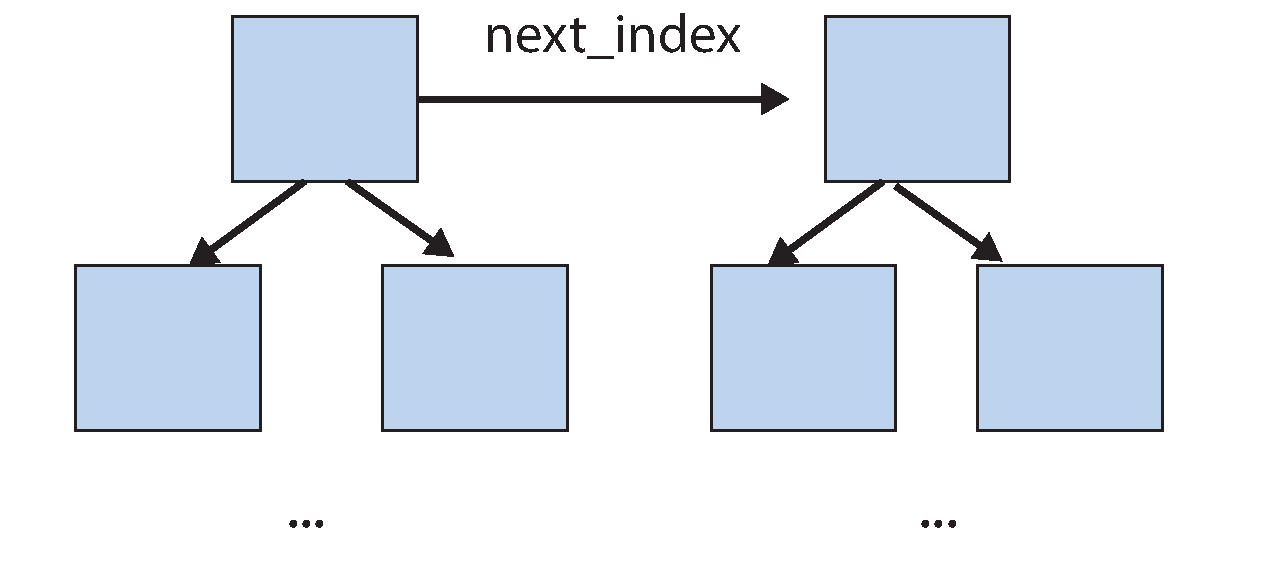
\includegraphics[width=0.5\linewidth]{imgs/bvh.pdf}
    \caption{We use a stackless variant of Bounding Volume Hierarchy that stores an ``escape'' index per node. If a ray misses a node, we can skip all of its children and escape to the sibling.}
    \label{fig:bvh}
\end{figure}

We will explain the idea of bounding volume hierarchies in lectures. Or you can read the \href{https://raytracing.github.io/books/RayTracingTheNextWeek.html#boundingvolumehierarchies}{ray tracing book} for some ideas as well. Due to the limitation that we cannot implement recursion, we will implement a \href{https://www.cse.chalmers.se/edu/course.2016/course/TDA361/EfficiencyIssuesForRayTracing.pdf}{\emph{stackless} variant} of bounding volume hierarchy traversal. The idea is to flatten the hierarchy nodes into a contiguous array in a pre-order tree visit order. For each node with index $i$, we store its the index of the first node after the entire sub-tree below $i$ in \lstinline{next_index}. Because we store the items in pre-order, all nodes between \lstinline{[i, next_index)} are the descendants of node $i$. Therefore if a ray misses node $i$, we can skip this entire range and move our bounding volume hierarchy traversal to the next index. If a ray hits a node $i$, we can simply traverse the next node $i+1$ which corresponds to a Depth-First-Search of the tree.
For a root node, we set its \lstinline{next_index} to the end of the nodes, so you can use it as an indicator for reaching the end.

If a node is a leaf node, it may contain one-to-four triangles, with indices stored in \lstinline{triangle_begin} and \lstinline{triangle_end}. Loop over these indices to check all triangles inside. 

We further flatten all bounding volume hierarchies of all meshes into a single contiguous array \lstinline{StructuredBuffer<BVHNode> bvh_nodes}. Each triangle mesh has a member \lstinline{bvh_root_index} that you can look into where the root is in the global array.

For the bounding volumes, we use Axis-Aligned Bounding Boxes. We have provided the ray-axis-aligned-bounding-box intersection code in \lstinline{intersect_aabb} in \lstinline{hw3_common.slang}.

We have also provided the host hierarchy construction code for you. See \lstinline{build_bvh} in \lstinline{hw3_scene.py}. 

Go to \lstinline{hw3_6.slang} and replace your triangle mesh intersection code with bounding volume hierarchy traversal code. 
Test it using
\begin{lstlisting}[language=bash]
    uv run python main.py 3_6 scenes/hw3/dragon.json
\end{lstlisting}

I have put my rendering in \cref{fig:hw3_6}.
\begin{figure}[h]
    \centering
    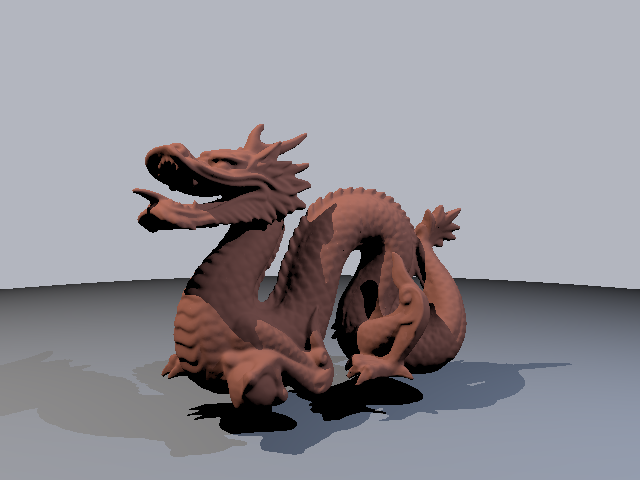
\includegraphics[width=0.5\linewidth]{imgs/hw_3_6.png}
    \caption{Reference rendering for homework 3.6.}
    \label{fig:hw3_6}
\end{figure}

We will grade your renderer using the following commands.
\begin{lstlisting}[language=bash]
    uv run python main.py -output outputs/hw_3_6_1.png 3_6 scenes/hw3/dragon_2.json
    uv run python main.py -output outputs/hw_3_6_2.png 3_6 scenes/hw3/bunny.json
    uv run python main.py -output outputs/hw_3_6_3.png 3_6 scenes/hw3/trio.json
    uv run python main.py -output outputs/hw_3_6_4.png 3_6 scenes/hw3/ritual.json
    uv run python main.py -output outputs/hw_3_6_5.png 3_6 -time 6.2 scenes/hw3/50_flying_dragons.json
\end{lstlisting}
The last scene has 50 Stanford dragon, which is roughly 50 millions of triangles! It shows the power of instancing (applying different transformations to the same mesh) and bounding volume hierarchies.

Note that the ray tracer is identical to 3.5 except for how we find the closest triangle intersection. The resulting image should be exactly the same, but the rendering time should be dramatically shorter.

\section{Make your own scene (5 points)}

As usual, design a scene yourself and submit the scene and your rendering to us. Feel free to download 3D model files on the internet (please credit the authors and let us know where you downloaded it). Note that our scene/mesh format may not be fully compatible with what you downloaded.
Please also submit all meshes referenced by your scene, so that we can reproduce your rendering.

\end{document}